\subsection{Strict Validation, External Validation, and Capability Boundaries}

The stricter protocols reduced fixed chronological performance and changed the numerical ordering of the complete five-class models. Across five seeds under the 14-window purged protocol, Stage 1 AUPRC was $0.6006 \pm 0.0062$, Stage 2 Macro-F1 was $0.7944 \pm 0.0049$, Cascade Macro-F1 was $0.5683 \pm 0.0177$, and Direct Five-Class Macro-F1 was $0.6024 \pm 0.0049$. The paired Direct-minus-Cascade difference was 0.0340, with a flight-log-bootstrap 95\% CI of $[-0.0047, 0.0762]$. The mean ordering reversed relative to the fixed chronological split, but the paired interval included zero and therefore did not support a stable purged-protocol advantage. Figure~\ref{fig:protocol_robustness} summarizes these protocol-level comparisons.

Leave-log-out evaluation assigned complete logs to the partitions, with 970 logs for training, 206 for validation, and 213 for testing. Across five seeds, Stage 1 AUPRC was $0.6296 \pm 0.0023$ and AUROC was $0.9265 \pm 0.0008$. At the validation-derived operating threshold, Stage 1 F1 was $0.5989 \pm 0.0042$ and log-aware event F1 was $0.4533 \pm 0.0241$. The anomaly-only Stage 2 LightGBM classifier achieved Macro-F1 of $0.9041 \pm 0.0029$ and Balanced Accuracy of $0.8876 \pm 0.0040$. On the complete five-class task, the Cascade achieved Macro-F1 of $0.5962 \pm 0.0048$ and Balanced Accuracy of $0.5840 \pm 0.0057$, while Direct Five-Class achieved Macro-F1 of $0.6092 \pm 0.0043$ and Balanced Accuracy of $0.6341 \pm 0.0022$.

The paired Direct-minus-Cascade Macro-F1 difference under leave-log-out was 0.0130, with a flight-log bootstrap 95\% confidence interval of $[-0.0282, 0.0438]$ based on 1000 repetitions. Because the interval includes zero, these results do not support a stable performance difference or a general performance advantage for the hierarchical Cascade. The Cascade remains a distinct gated decision structure, but its fixed-split performance ordering should not be interpreted as a protocol-independent superiority.

The ALFA experiment evaluated zero-shot binary anomaly detection using 16 semantically shared physical channels and a threshold fixed from UAV-SEAD validation data. On 46 ALFA sequences and 5273 ALFA windows, the transferred detector obtained AUPRC of $0.3181 \pm 0.0086$ and AUROC of $0.6679 \pm 0.0069$. The ALFA faults were not mapped to the four UAV-SEAD fault domains; these values therefore assess binary score transfer only. The separate flight-level screening of 139 Uncategorized logs against 898 pure-Normal logs produced flight-level AUPRC of $0.2784 \pm 0.0046$, AUROC of $0.6610 \pm 0.0049$, F1 of $0.3307 \pm 0.0142$, Uncategorized recall of $0.4118 \pm 0.0314$, and Normal specificity of $0.8575 \pm 0.0073$. Because Uncategorized annotations have no temporal ranges, this screening does not support point-wise or event-level claims.

The controlled PX4 replay provided the only module-level ground truth, but its evaluation exposed a detector-gated capability boundary. In the onset-conditioned bidirectional analysis, which supplied the known 30-s injection time and used matched baseline evidence, overall Top-1, Top-3, and Top-5 recalls were 0.250 (95\% two-way cluster-bootstrap CI [0.000, 0.583]), 0.333 [0.000, 0.750], and 0.333 [0.000, 0.750], respectively. MRR was 0.3227 [0.0455, 0.6790], and mean EXAM was 0.3318 [0.1065, 0.5772]. These intervals independently resample the three source logs and four mutation types and remain wide because both cluster counts are small. The conditional ranks were uneven across mutations: EKF2 innovation bias reached Top-1 in two of three runs, whereas INAV local-z freeze and Land Detector state inversion did not enter Top-5 in any run. These results quantify conditional ranking behavior after onset information is supplied.

The unchanged real-flight Stage 1 detector, however, detected 0 of 12 controlled mutation runs at its fixed threshold of 0.3374776883. Consequently, detector-gated Top-1, Top-3, Top-5, and MRR were all zero; detection delay and detector-gated ranking delay were undefined. Figure~\ref{fig:replay_gated_boundary} contrasts the onset-conditioned and detector-gated metrics. The onset-conditioned values must therefore not be presented as end-to-end software-module localization performance. Taken together, the replay results support conditional software-module suspect ranking while identifying real-flight-to-replay domain shift as a current limit of the complete evidence chain.

\begin{figure}[H]
    \centering
    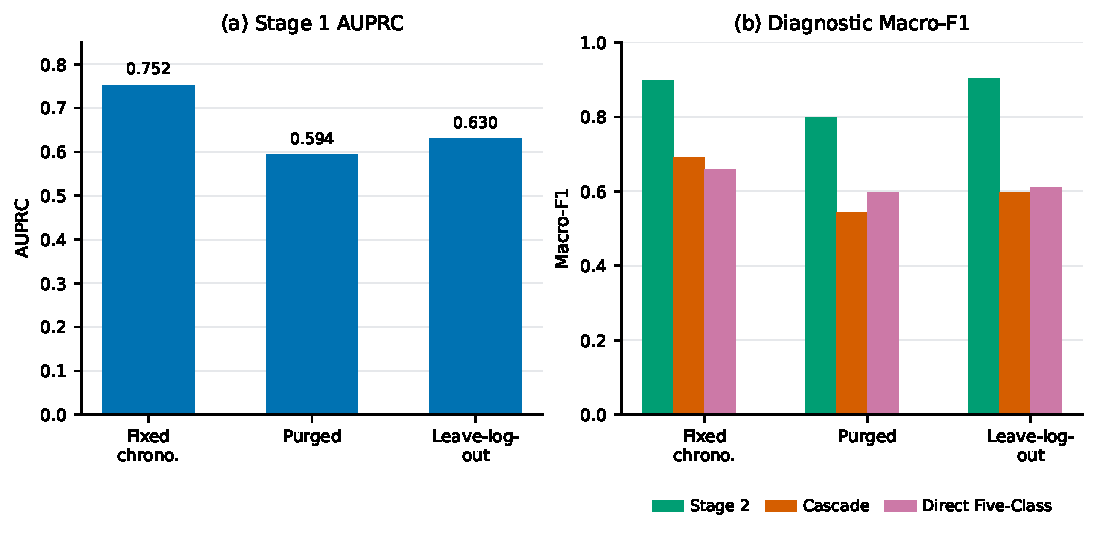
\includegraphics[width=\textwidth]{figures/figure_3_protocol_robustness.pdf}
    \caption{Primary protocol comparison for Stage 1 detection and complete or conditional diagnosis. The fixed chronological, purged, and leave-log-out protocols are evaluated with their respective split definitions; error bars show standard deviations across five seeds. Purging reverses the mean ordering of Cascade and Direct Five-Class Macro-F1, but the paired flight-log interval for their difference includes zero.}
    \label{fig:protocol_robustness}
\end{figure}

\begin{figure}[H]
    \centering
    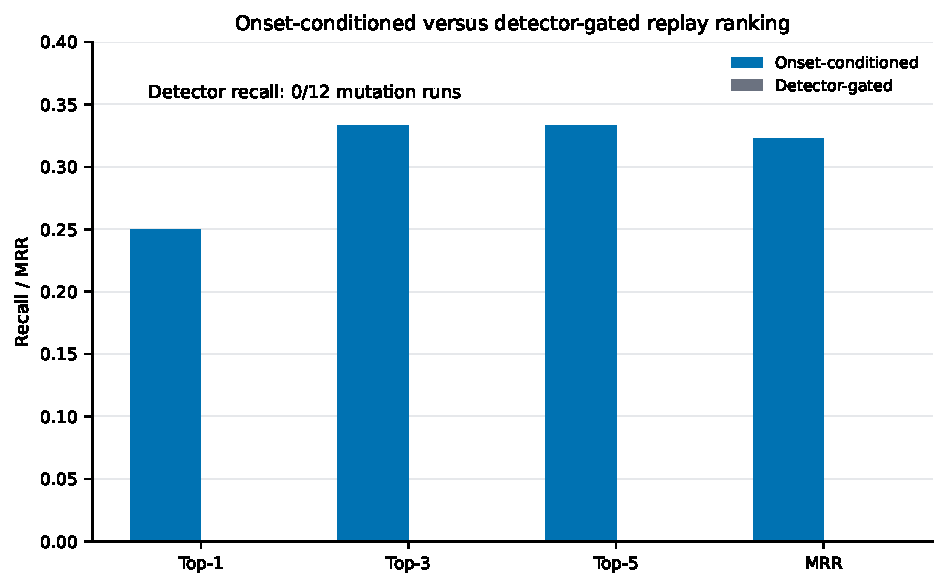
\includegraphics[width=\textwidth]{figures/figure_5_replay_onset_vs_detector_gated.pdf}
    \caption{Controlled PX4 replay module-ranking metrics under two evaluation layers. Onset-conditioned ranking uses the known injection time and matched baseline evidence; detector-gated ranking first requires the unchanged real-flight Stage 1 detector to fire. The detector-gated recall was 0/12 for the evaluated mutation runs.}
    \label{fig:replay_gated_boundary}
\end{figure}
